%!TEX root = origin_elements_lecture_notes.tex

\chapter{The Life and Death of the Sun}

In the last chapter we have seen how stars form from molecular clouds. We also derived the hydrostatic equilibrium, which is the conditions that stars spend most of their life in, and have analyzed some of its consequences. While we have already determined some key facts about the Sun, in this chapter we discuss the life of the Sun, its place among other stars in the Milky Way, and its ultimate fate in more detail. Understanding the Sun is useful; after all it is the energy source required for life on Earth. However, the Sun is also regularly used in comparison with other stars when discussing their lifetimes and fates.

\section{The Sun's Place in the Milky Way}

In Chapter~\ref{ch:solar_system_abundnaces} we have already discussed the place of the Sun in the Milky Way, see, e.g., Figure~\ref{fig:milky_way_profile_wiki}. Here, we will now also have a more detailed look at the Sun with respect to other stars -- its neighbors -- in the galaxy.

\subsection{The Hertzsprung-Russell Diagram}

\begin{figure}[p]
    \centering
    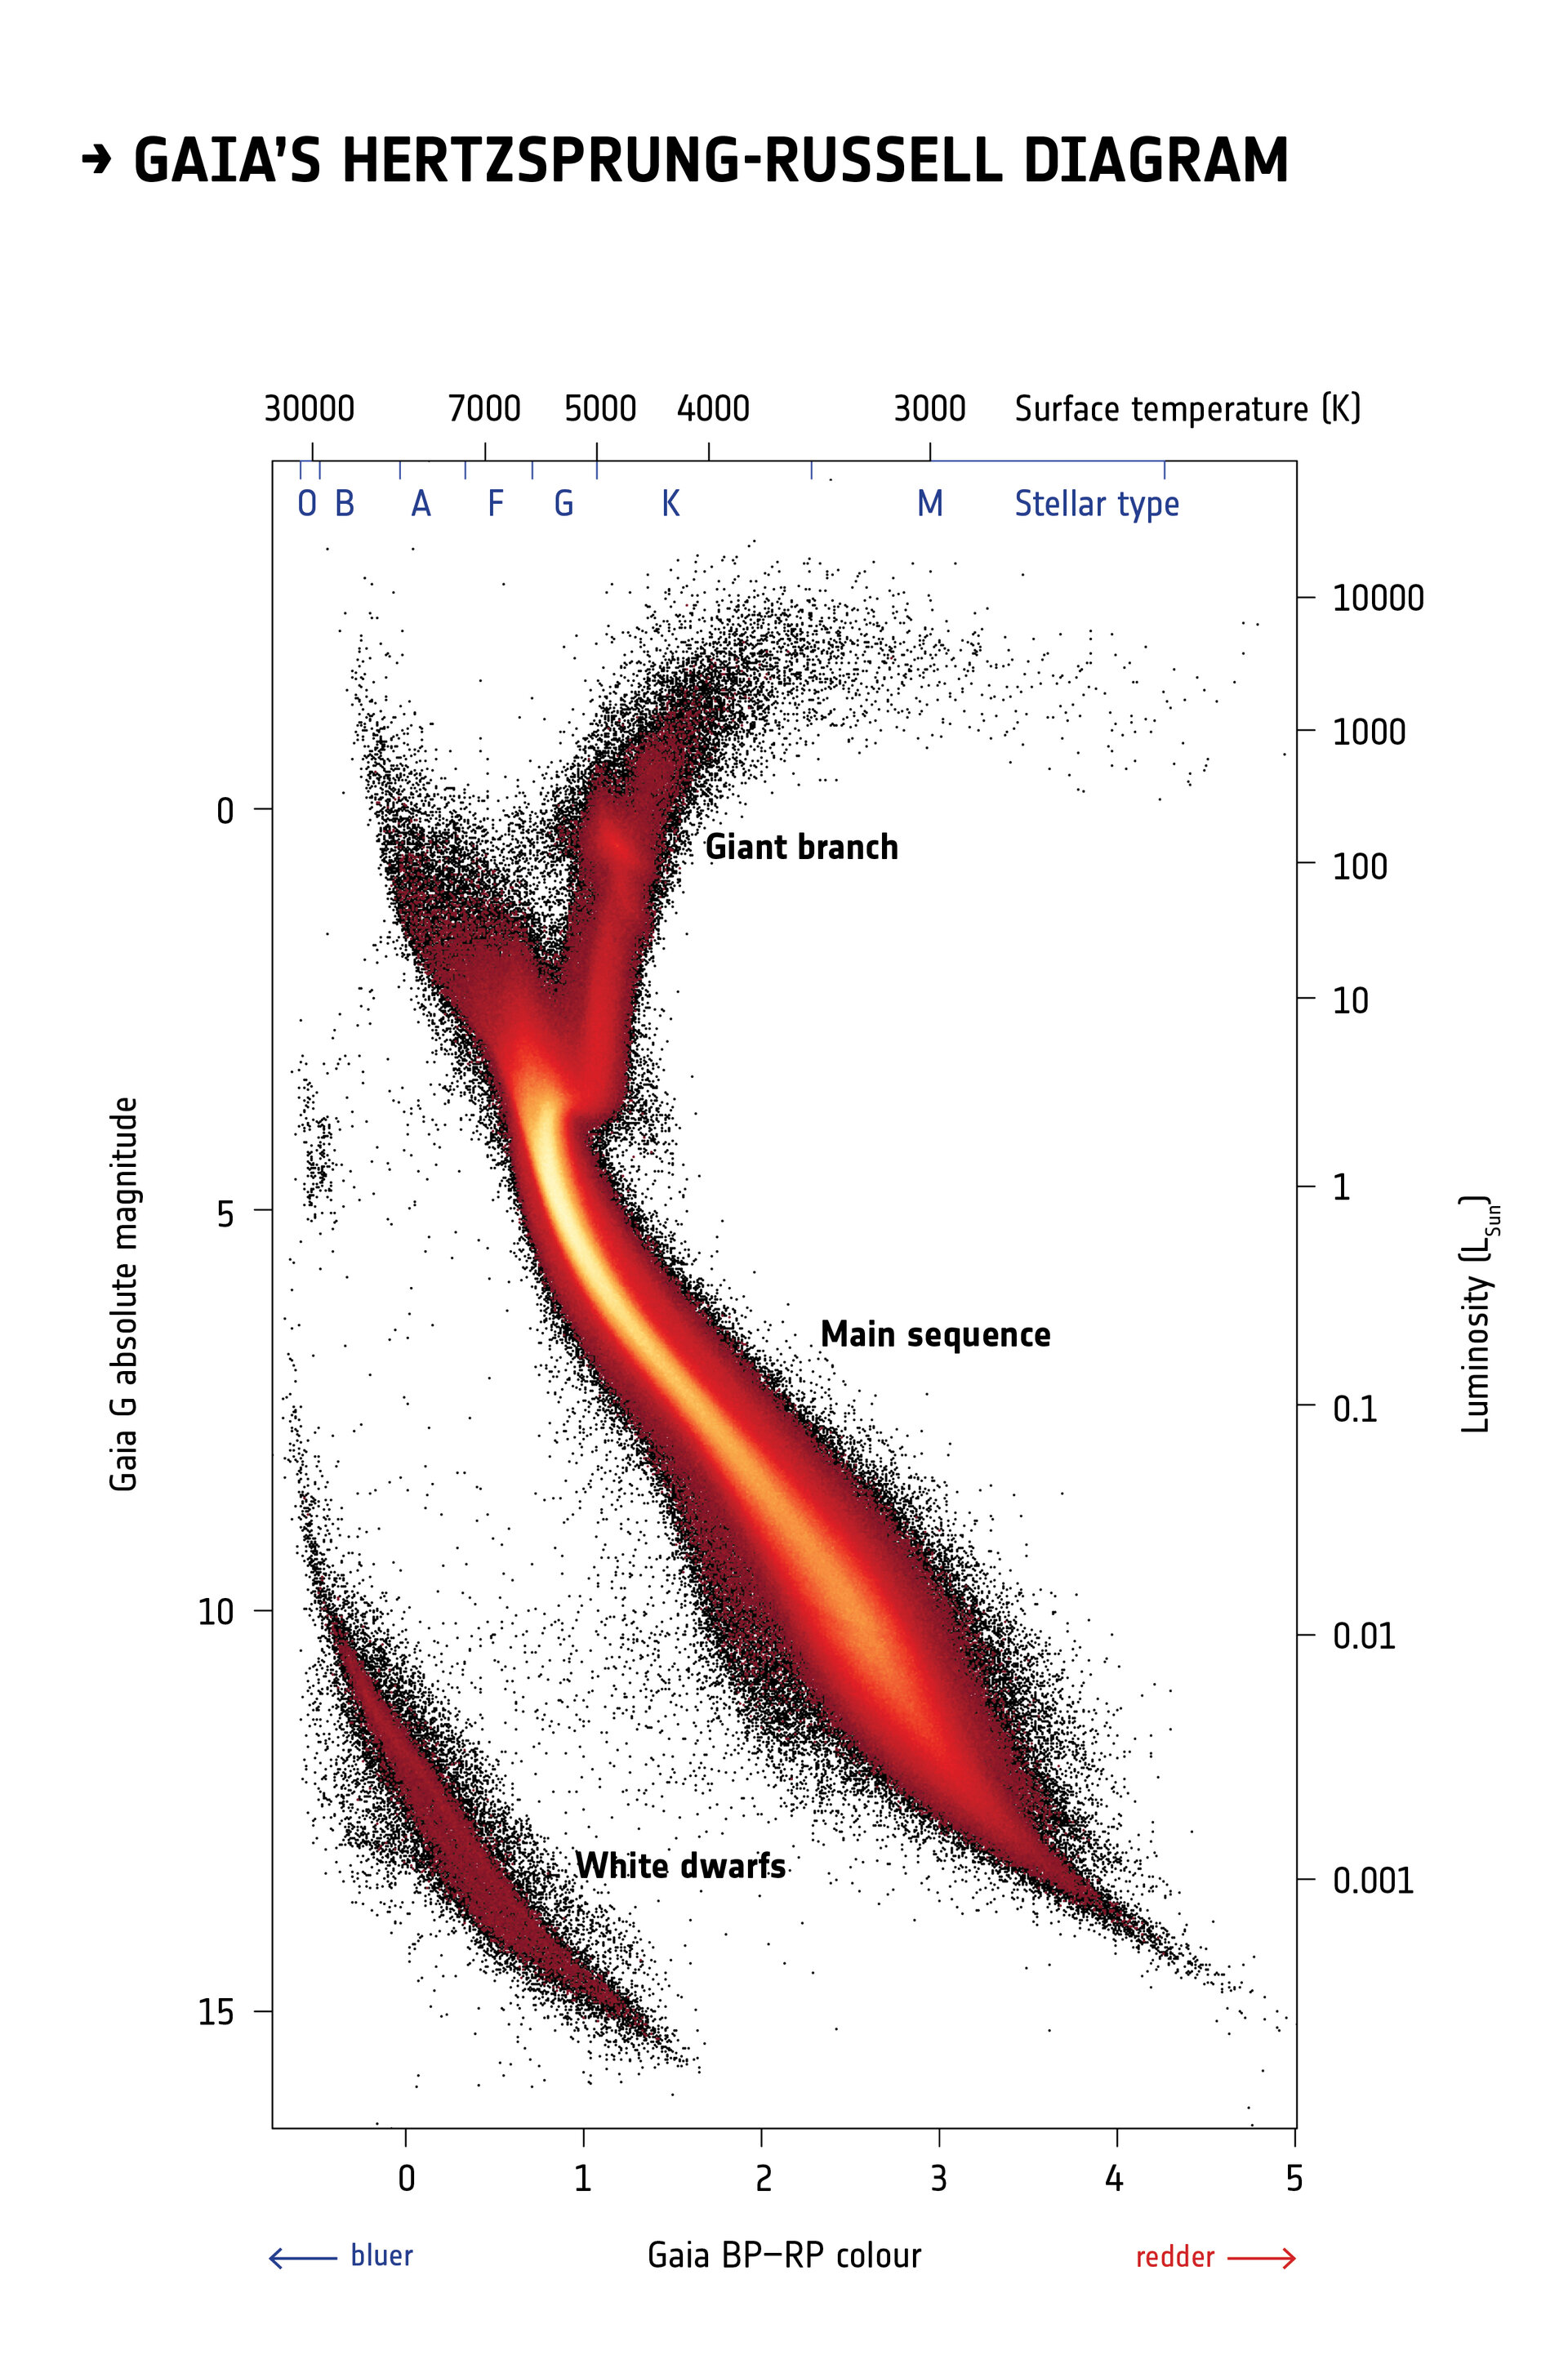
\includegraphics[width=0.81\textwidth]{graphics/sun/gaia_hrd}
    \caption{The \acl{hrd} put together from four million stars within 5000\,ly of the Sun. Credit: \acs{esa}/Gaia/DPAC, CC BY-SA 3.0 IGO.}
\label{fig:sun:hrd_gaia}
\end{figure}

Large-scale photographic and spectroscopic observations of stars led in the early 19$^\mathrm{th}$ century to the assembly of the first \ac{hrd}. An updated version of this diagram that includes around four million stars within 5000\,ly of the Sun is shown in Figure~\ref{fig:sun:hrd_gaia}. The observations for this \ac{hrd} were done with \href{https://sci.esa.int/web/gaia}{Gaia}, a space mission by the \ac{esa}. 

The \ac{hrd} originally showed the magnitude of a star, i.e., its brightness, versus its stellar type. While the brightness is directly related to the luminosity, the stellar type is related to the peak in its spectrum and thus to the star's surface temperature. Wien's displacement law (see Section~\ref{sec:solar_system_abundances:the_sun}) allows us to directly correlate the stellar type with the surface temperature of a star. Thus, the \ac{hrd} diagram plots the luminosity of a star, usually normalized to the solar luminosity $L_\odot$, with respect to its surface temperature.

Various notations exist for stellar types, see, e.g., \href{https://en.wikipedia.org/wiki/Stellar_classification}{here}. In Figure~\ref{fig:sun:hrd_gaia} the Harvard system is used, in which the stellar types from hottest to coldest stars are O, B, A, F, G, K, M (see the top axis of Figure~\ref{fig:sun:hrd_gaia}).

The Sun has a surface temperature of around $5800$\,K and is thus a G-type star. Knowing it's luminosity ($1\,L_\odot$), it's position in the \ac{hrd} can be identified. The Sun lays centered on a branch in the \ac{hrd} that is labeled as main sequence. The main sequence is the location in the \ac{hrd} where stars spend their lives, i.e., their quiescent burning phases. Once the nuclear fuel is exhausted, stars collapse further until the next burning stage can be activated. At this point, stars expand while keeping their surface temperature similar, thus they significantly increase their luminosity and wander up onto the giant branch. Finally, low mass stars end up as so-called \acp{wd}. These objects, usually surrounded by planetary nebulae, are compact and hot. Due to their small size, their luminosity is fairly low, which places them in the bottom left corner of the \ac{hrd}.

% \subsection{The Mass-Luminosity Relation}

\subsection{Planetary Systems}

With the discovery of the first exoplanet in 1995 by Michel Mayor and Didier Queloz of the Geneva Observatory, the Sun was suddenly not the sole star anymore that had planets orbiting it. The existence of other planets outside the Solar System has been long suspected; it is thought that Giordano Bruno (1548-1600), a Dominican monk, believed in a Copernican universe filled with an infinite number of inhabited worlds around other stars. While no evidence exists at this point for inhabited worlds, multiple exoplanets in the so-called Goldilocks or habitable zone have been discovered. These rocky planets are located at a distance from their parent star that allows for the existence of liquid water on the surface, like Earth. Note that while Mayor and Queloz received the 2019 Nobel Prize,\footnote{\url{https://www.nobelprize.org/prizes/physics/2019/summary/}} Bruno was executed for his beliefs. 

According to NASA's exoplanet website,\footnote{\url{https://exoplanets.nasa.gov/}} the current number of confirmed exoplanets as of \ExoplanetDate\ is \ExoplanetsNumber.
\begin{figure}[tb]
    \centering
    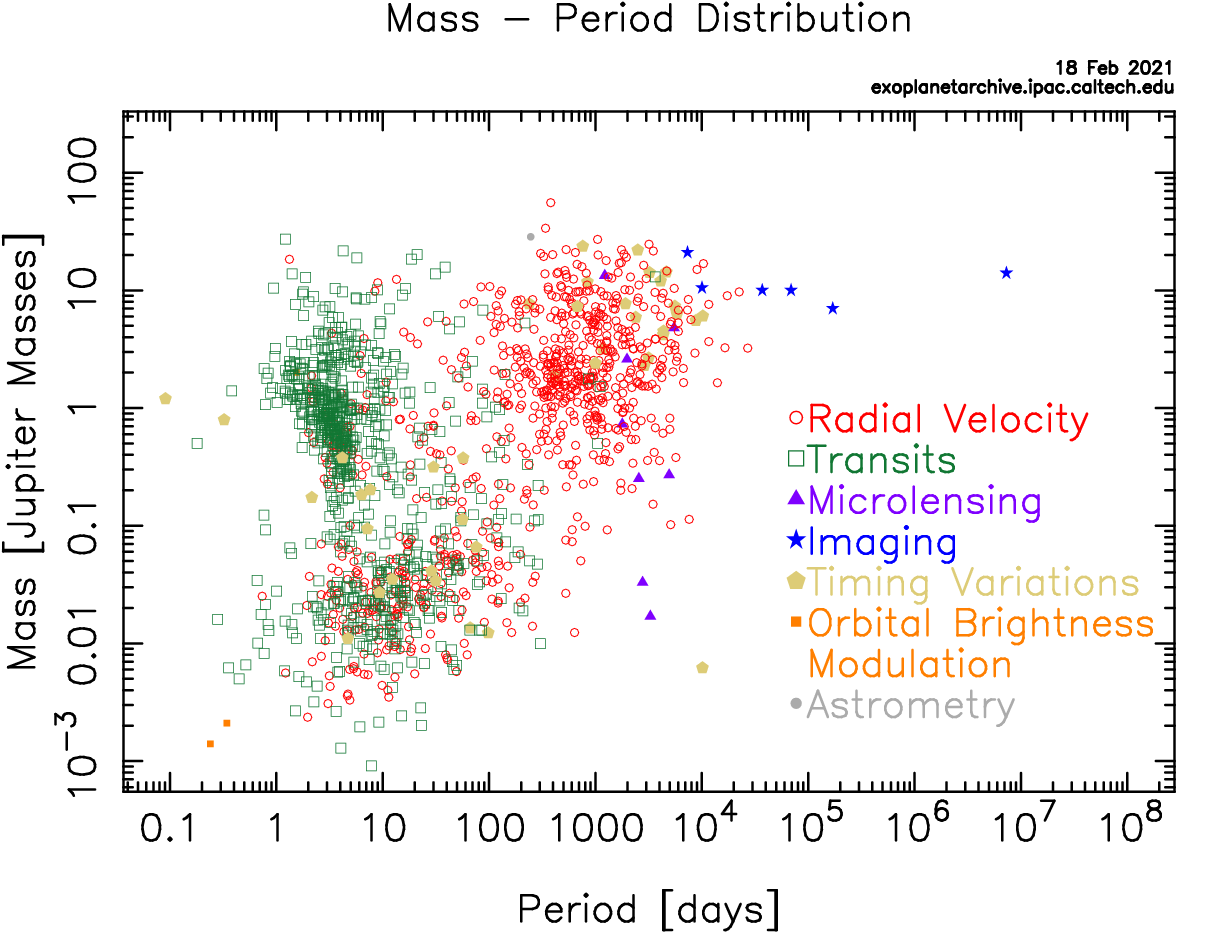
\includegraphics[width=0.75\textwidth]{graphics/sun/exoplanets_radius_period}
    \caption{Size of discovered expolanets as a function of their orbital periods. Source: \href{https://exoplanetarchive.ipac.caltech.edu/}{Exoplanet Archive, IPAC, Caltech}.}
    \label{fig:sun:exoplanets}
\end{figure}
Figure~\ref{fig:sun:exoplanets} shows a current figure for the size of confirmed exoplanets as a function of their orbital period. The size here is given in multiples of the size of Jupiter ($\jupiter$). Note that Earth ($\earth$) in this figure would plot at $M_{\earth} = 3.15 \times 10^{-3} M_{\jupiter}$ and at a period of 365\,d. Jupiter itself on the other hand, in comparison to other exoplanets, has an orbital period of 4333\,d. This shows that the Solar System seems to be an outlier when compared to all discovered exoplanets. Many of these exoplanets are heavy and orbit their parent star at short distances. Some massive exoplanets have orbital periods of a day and shorter. To what extent these discrepancies are due to observational bias remains under investigation, see, e.g., \citet{mulders18} and \citet{mulders19}.

\begin{table}[b]
\codebox{The Expolanet Population Observer Simulator (EPOS)}{is a python software package to simulate observations of expolanet populations. This package allows to study observational biases in transit and radial velocity exoplanet surveys, e.g., when analyzing data from the \href{https://www.nasa.gov/mission_pages/kepler/main/index.html}{Kepler} mission. The software package is well documented on \href{https://epos.readthedocs.io/en/latest/}{Read the Docs} and its source is available on \href{https://github.com/GijsMulders/epos/}{GitHub}.}
\end{table}


\subsection{Is the Sun Special?}

The Sun, overall, seems to be an average star like many others. While it plots in warmer areas of the \ac{hrd} than most stars that are on the main sequence, see Figure~\ref{fig:sun:hrd_gaia}, it is not outstandingly hot or cold. With respect to its planetary system it remains to be seen how common the Solar System as a whole is. Comparing the Solar System to exoplanets (Figure~\ref{fig:sun:exoplanets}) it seems as if we are fairly unique, however, this could simply be the result of observation biases since it is currently difficult to detect Earth-sized planets that orbit their parent star at distances of 1\,AU from their parent star. However, the habitable zone of a star of course does not just depend on the distance but also on the star's luminosity. 

The Sun is special in one aspect that has not been discussed so far, namely, it does not have a companion star. More than half of all stars are part of multiple star systems. As we will see later, these systems can have a significant effect on the stellar evolution and nucleosynthesis, and in some cases even be crucial for the production of certain elements.



\section{The Sun's Quiescent Burning Phase}

After having formed from a collapsing molecular cloud, the Sun entered the main sequence of the \ac{hrd} once nuclear fusion of hydrogen became the dominant heat source. Astronomers also refer to a star at the point when it enters the main sequence as a \ac{zams} star. From here on, the quiescent burning phase starts, in which stars slowly fuses hydrogen to helium. The \ac{hrd} in Figure~\ref{fig:sun:hrd_gaia} shows that most stars lay on the main sequence. The reason for this is that hydrogen burning is the longest phase a star goes through.

The four-body reaction 4 \ex{1}H \textrightarrow\ \ex{4}He + $\gamma$ is extremely unlikely to happen. Hydrogen fusion rather takes place in stages. Multiple processes are responsible as outlined below.

\subsection{The Proton-Proton-Chain}

\begin{figure}[tb]
    \centering
    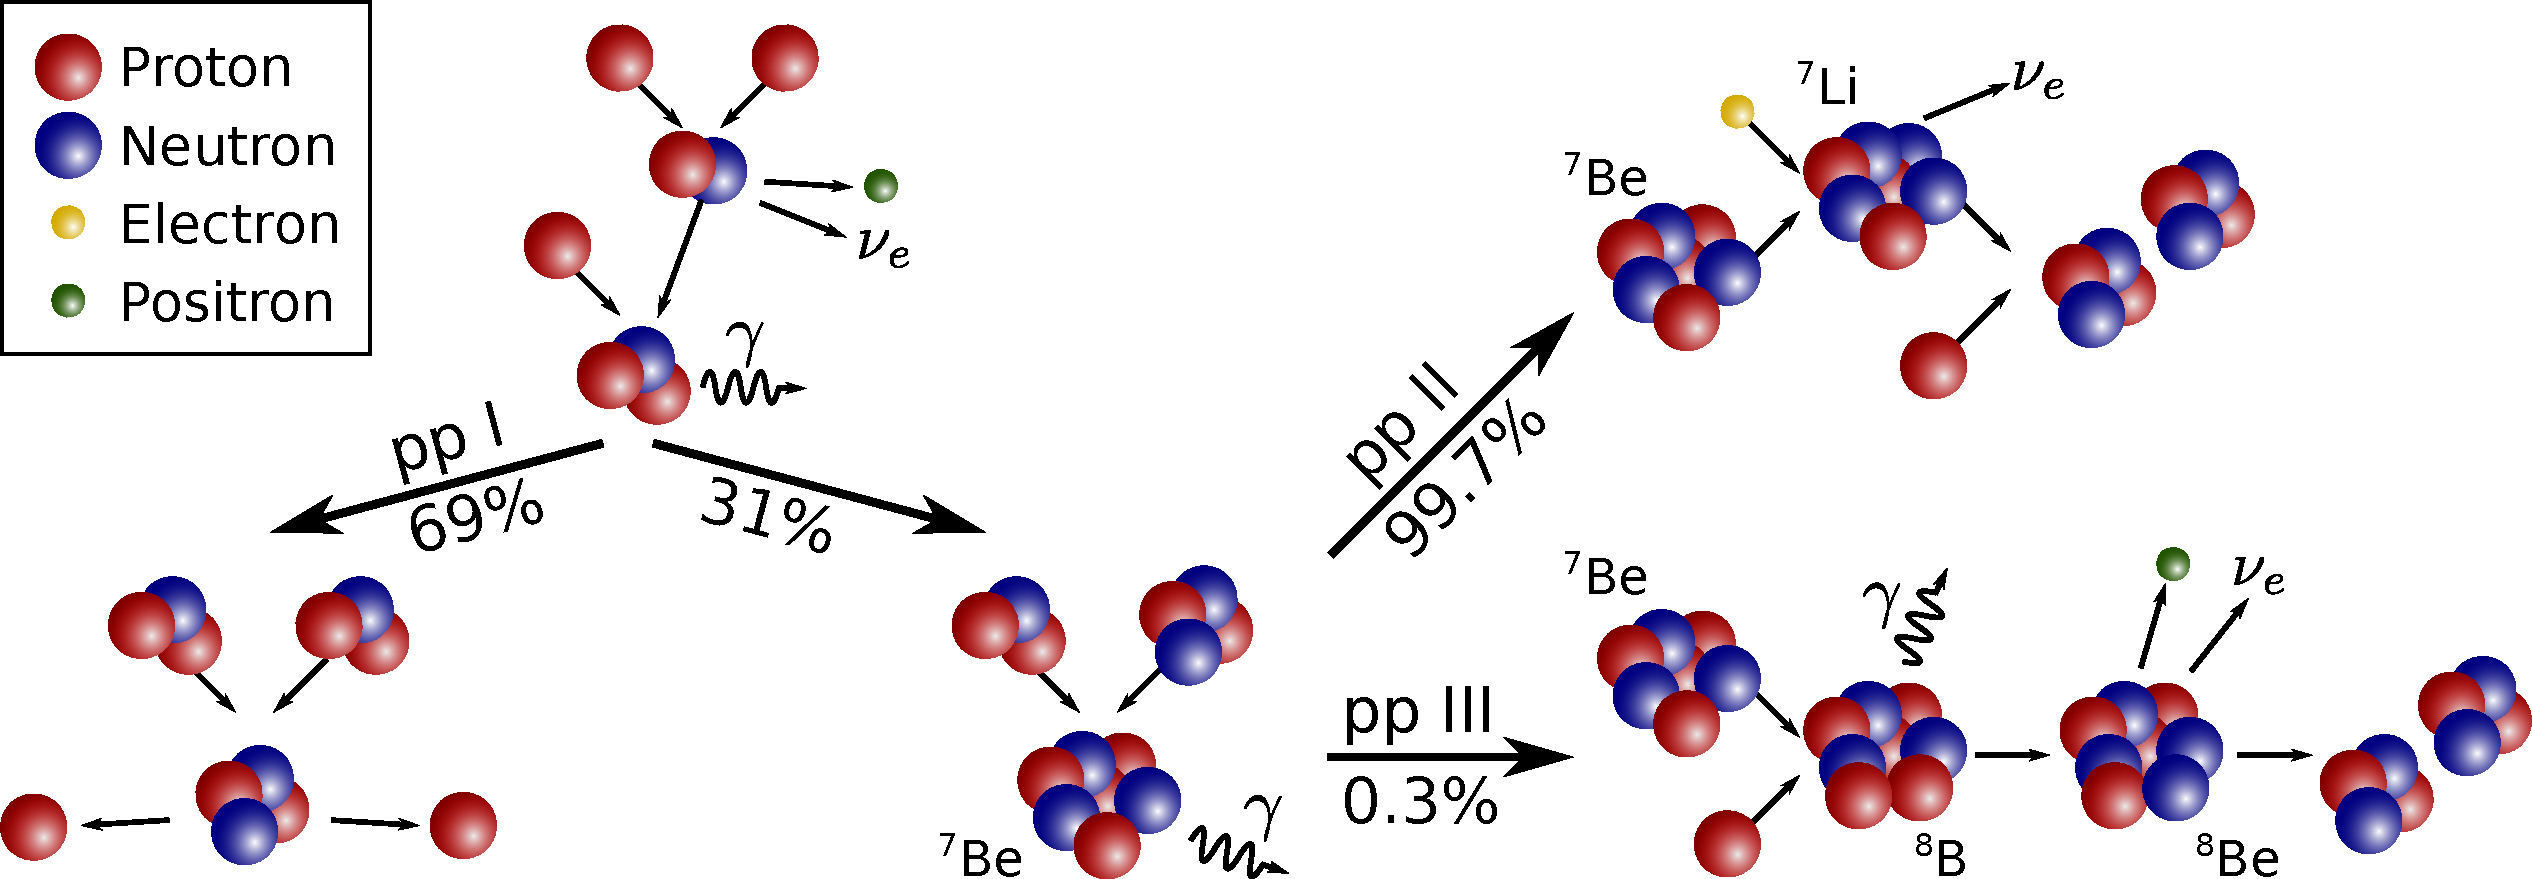
\includegraphics[width=\textwidth]{graphics/sun/pp_chain}
    \caption{The \ac{pp-chain} and it's three branches. Percentages are with respect to hydrogen fusion in the Sun.}
    \label{fig:sun:pp-chain}
\end{figure}
The \ac{pp-chain} is the main reaction chain that fuses hydrogen to helium in the Sun. Figure~\ref{fig:sun:pp-chain} shows a schematic of the \ac{pp-chain} and its three main branches. All branches start out with the reactions
\begin{align}
    {^1}\mathrm{H} + {^1}\mathrm{H} &\longrightarrow {^2}\mathrm{H} + \nu_e + e^+ \\
    {^2}\mathrm{H} + {^1}\mathrm{H} &\longrightarrow {^3}\mathrm{He} + \gamma.
\end{align}
Three protons are thus converted via deuterium (\ex{2}H) into a \ex{3}He nucleus. At this point the \ac{pp-chain} branches. The pp I chain, which is responsible for 69\% of the energy produced in the Sun via the \ac{pp-chain}, fuses two \ex{3}He nuclei and forms one \ex{4}He nucleus in the
\begin{equation}
    {^3}\mathrm{He} + {^3}\mathrm{He} \longrightarrow {^4}\mathrm{He} + 2\,{^1}\mathrm{H}
\end{equation}
reaction.

On the other branch in the \ac{pp-chain}, which takes place 31\% of the time in the Sun, a \ex{3}He and a \ex{4}He nuclei are first combined to form \ex{7}Be. The reaction is
\begin{equation}
    {^3}\mathrm{He} + {^4}\mathrm{He} \longrightarrow {^7}\mathrm{Be} + \gamma. \label{eqn:sun:pp-chain:intermediate_second_branch}
\end{equation}
Two paths are possible from here. The pp II chain forms \ex{4}He via the following reactions from \ex{7}Be:
\begin{align}
    {^7}\mathrm{Be} + e^{-} &\longrightarrow {^7}\mathrm{Li} + \nu_e \\
    {^7}\mathrm{Li} + {^1}\mathrm{H} &\longrightarrow 2\,{^4}\mathrm{He}
\end{align}
The \ex{4}He nucleus that is consumed in reaction~\eqref{eqn:sun:pp-chain:intermediate_second_branch} is gained back in the end. The pp II chain takes place 99.7\% of the time after the first branching.

The rest of the time in this second branch, the pp III chain produces \ex{4}He from \ex{7}Be. The reactions that take place are as following:
\begin{align}
    {^7}\mathrm{Be} + {^1}\mathrm{H} &\longrightarrow {^8}\mathrm{B} + \gamma \\
    {^8}\mathrm{B} &\longrightarrow {^8}\mathrm{Be} + e^+ + \nu_e\\
    {^8}\mathrm{Be} &\longrightarrow 2\,{^4}\mathrm{He}
\end{align}
The latter two reactions are here simply the decays of \ex{8}B and \ex{8}Be to form two \ex{4}He. Thus, the \ex{4}He consumed after the first branching is again gained back plus an additional \ex{4}He forms.

The nuclear energy generation rate in W\,kg$^{-1}$, simplified after equation~(10.46) in \citet{carroll17} (page 311), can be written as
\begin{equation}
    \epsilon_\mathrm{pp} = 0.241 \rho X^2 T_6^{-\nicefrac{2}{3}} \exp\left(-33.8 T_6^{-\nicefrac{1}{3}}\right). \label{eqn:sun:energy_generation_pp-chain}
\end{equation}
Here, $\rho$ is the density of the star's center and $T_6$ is the temperature expressed in multiples of $10^6$\,K. Assuming a density in the center of the Sun of $\rho = 150\,\mathrm{g}\,\mathrm{cm}^{-2}$, we can calculate the energy production of the \ac{pp-chain} at $\epsilon_\mathrm{pp} = 3.4 \times 10^{-3}\,$W\,kg$^{-1}$.


\subsection{The CNO-Cycle}
\begin{figure}[tb]
    \centering
    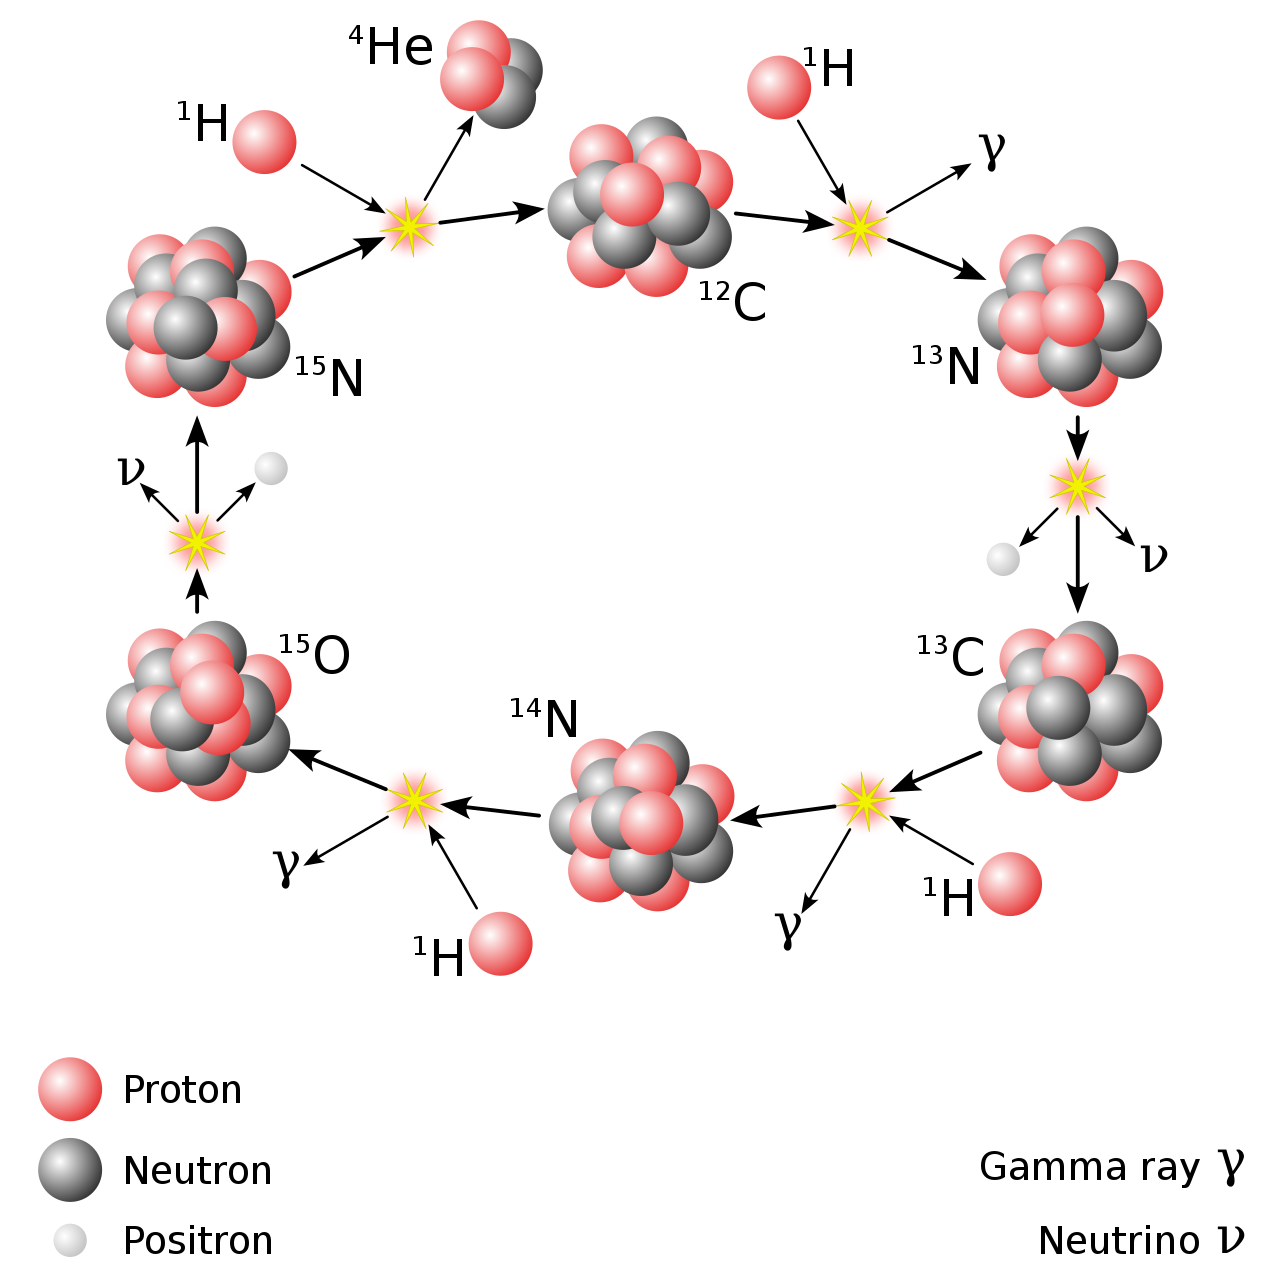
\includegraphics[width=0.6\textwidth]{graphics/sun/cno_cycle}
    \caption{Schematic drawing of the CNO cycle and the involved reactions. A \ex{4}He nucleus forms by combining four protons. The elements carbon, nitrogen, and oxygen act as catalysts for the reactions. Credit: \href{https://en.wikipedia.org/wiki/CNO_cycle}{Wikipedia}.}
    \label{fig:sun:cno_cycle}
\end{figure}
Compared to the \ac{pp-chain}, the CNO cycle requires carbon, nitrogen, and oxygen as catalysts for the reaction in order to combine four hydrogen nuclei into \ex{4}He. Figure~\ref{fig:sun:cno_cycle} shows a schematic of the CNO cycle. Starting at \ex{12}C, the involved reactions are as following:
\begin{align}
    {^{12}}\mathrm{C} + {^1}\mathrm{H} &\longrightarrow {^{13}}\mathrm{N} + \gamma\\
    {^{13}}\mathrm{N} &\longrightarrow {^{13}}\mathrm{C} + e^+ + \nu_e \\
    {^{13}}\mathrm{C} + {^1}\mathrm{H} &\longrightarrow {^{14}}\mathrm{N} + \gamma\\
    {^{14}}\mathrm{N} + {^1}\mathrm{H} &\longrightarrow {^{15}}\mathrm{O} + \gamma \label{eqn:sun:cno_cycle_n14_consumption}\\
    {^{15}}\mathrm{O} &\longrightarrow {^{15}}\mathrm{N} + e^+ + \nu_e\\
    {^{15}}\mathrm{N} + {^1}\mathrm{H} &\longrightarrow {^{12}}\mathrm{C} + {^4}\mathrm{He} \label{eqn:sun:cno_cycle_last_reaction}
\end{align}

As in the \ac{pp-chain}, the CNO cycle is also branched. This branch occurs at the last reaction~\eqref{eqn:sun:cno_cycle_last_reaction} and occurs only about 0.04\% of the time. The branch starting at reaction~\eqref{eqn:sun:cno_cycle_last_reaction}, which is not shown in Figure~\ref{fig:sun:cno_cycle}, is
\begin{align}
        {^{15}}\mathrm{N} + {^1}\mathrm{H} &\longrightarrow {^{16}}\mathrm{O} + \gamma\\
        {^{16}}\mathrm{O} + {^1}\mathrm{H} &\longrightarrow {^{17}}\mathrm{F} + \gamma\\
        {^{17}}\mathrm{F} &\longrightarrow {^{17}}\mathrm{O} + e^+ + \nu_e\\
        {^{17}}\mathrm{O} + {^1}\mathrm{H} &\longrightarrow {^{14}}\mathrm{N} + {^4}\mathrm{He}.
\end{align}
This branch thus does not drop back to \ex{12}C but rather produces \ex{14}N, which is also part of the CNO cycle and will be consumed further, see reaction~\eqref{eqn:sun:cno_cycle_n14_consumption}.

The nuclear energy generation rate in W\,kg$^{-1}$, simplified after equation (10.58) in \citet{carroll17} (page 312), can be written as
\begin{equation}
    \epsilon_\mathrm{CNO} = 8.67\times 10^{20} \rho X X_\mathrm{CNO} T_6^{-\nicefrac{2}{3}} \exp\left(-152.28 T_6^{-\nicefrac{1}{3}}\right). \label{eqn:sun:energy_generation_cno_cycle}
\end{equation}
Here, $X_\mathrm{CNO}$ is the mass fraction of CNO elements, i.e., the elements that are used as catalysts. In order for the CNO cycle to take place in a star, some metals must be present. For the Sun, the energy generation rate via the CNO cycle can be estimated as $\epsilon_\mathrm{CNO} = 2.3\times10^{-4}$\,W\,kg$^{-1}$.


\subsection{Energy Production in the Sun}

\begin{figure}[tb]
    \centering
    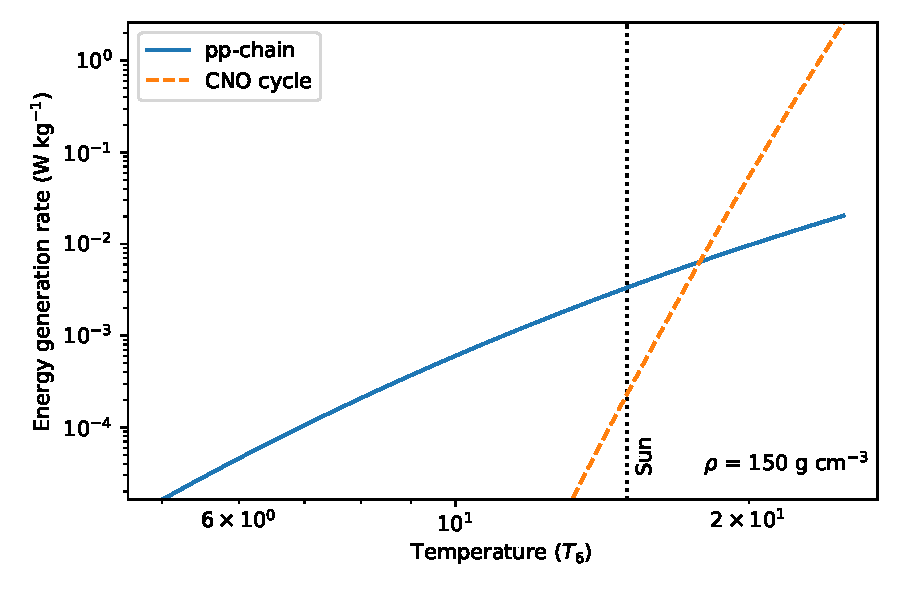
\includegraphics[width=0.75\textwidth]{graphics/sun/energy_h_burning}
    \caption{Energy generation rate due to the \ac{pp-chain} and CNO cycle as a function of temperature. The core density here is fixed to 150\,g\,cm$^{-3}$, which is approximately the density in the Sun's core.}
    \label{fig:sun:energy_generation_hydrogen_fusion}
\end{figure}
Figure~\ref{fig:sun:energy_generation_hydrogen_fusion} shows the energy generation rates of the \ac{pp-chain} and the CNO cycle (equations~\eqref{eqn:sun:energy_generation_pp-chain} and~\eqref{eqn:sun:energy_generation_cno_cycle}, respectively) as a function of the central temperature. A dotted line is shown at the Sun's central temperature. While the figure is scaled to the Sun's core density of $\rho\approx150$\,g\,cm$^{-3}$, both energy generation rates for the \ac{pp-chain} and the CNO cycle are proportional to $\rho$, thus the relative position of the two curves will stay the same for different stars and only depend on the temperature. 

Figure~\ref{fig:sun:energy_generation_hydrogen_fusion} clearly shows that the \ac{pp-chain} is the dominant energy source in the Sun. The CNO cycle's energy generation rate is more than an order of magnitude lower. However, at slightly higher temperatures, the CNO cycle will be the dominant source of nuclear energy that keeps a star in hydrostatic equilibrium.

In Section~\ref{sec:star_formation:first_stars} we discussed star formation at zero metallicity and concluded that these stars must have been very massive since cooling rates for molecular clouds are minimal at zero metallicity. If a star starts with $Z=0$, it can also only produce energy in its core via the \ac{pp-chain}. In Figure~\ref{fig:sun:energy_generation_hydrogen_fusion} it can be seen that the energy generation rate increases slower for the \ac{pp-chain} as a function of temperature compared to the CNO cycle. Thus, stars that start of with truly no metals must have gravitationally collapsed further until the temperature was high enough for the \ac{pp-chain} to compensate this infall and go into hydrostatic equilibrium.


\section{The Dying Sun}

\begin{figure}[bt]
    \centering
    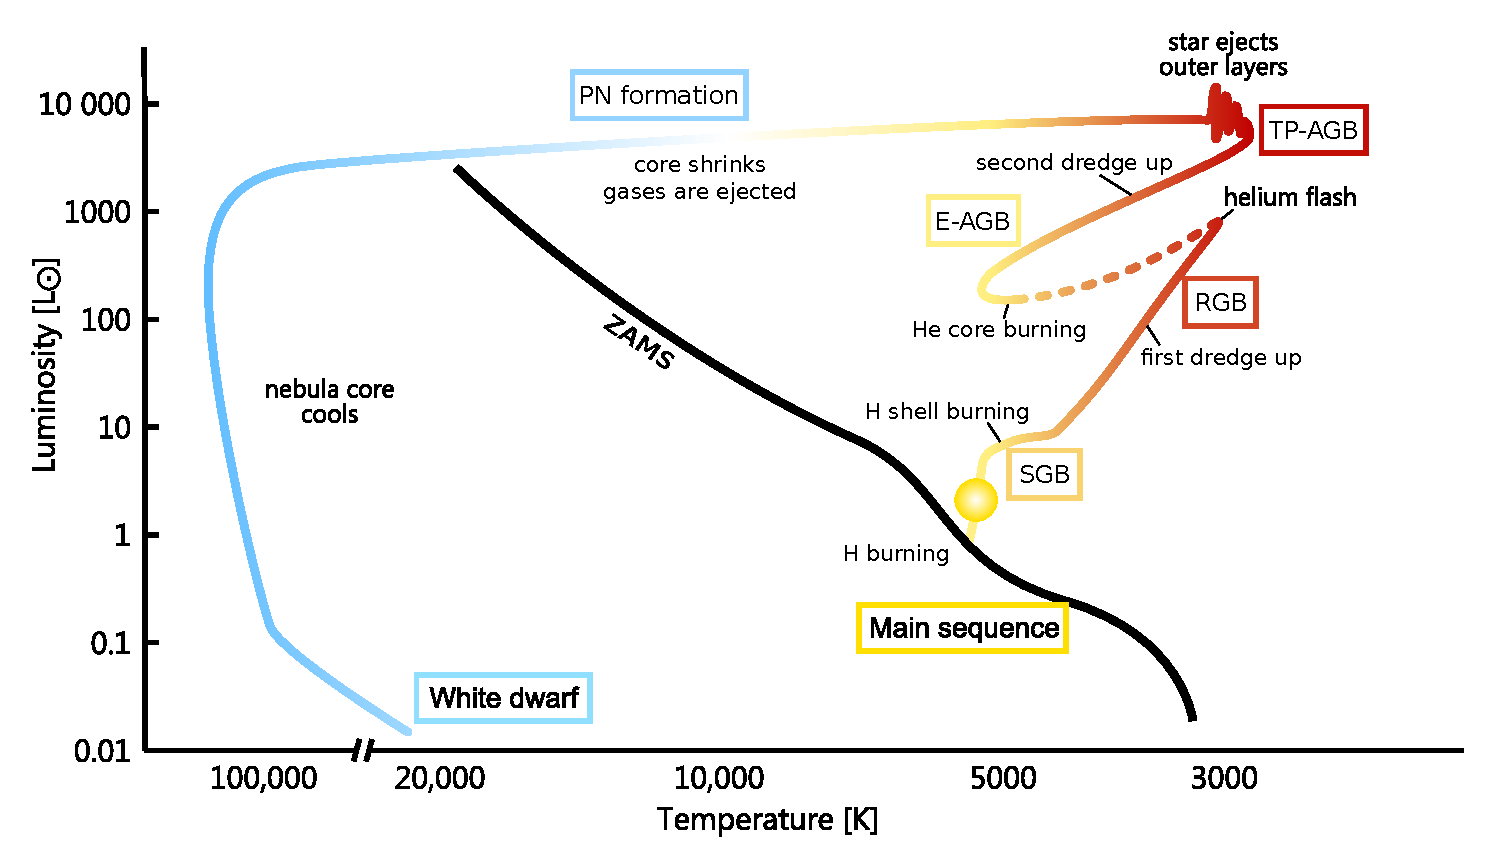
\includegraphics[width=0.9\textwidth]{graphics/sun/sun_hrd}
    \caption{Schematic of the evolution of the Sun in the \ac{hrd}. Figure adopted after \href{https://commons.wikimedia.org/wiki/File:Evolution_of_the_Sun_2_EN.svg}{Szczureq via Wikipedia Commons.}}
    \label{fig:sun:sun_hrd}
\end{figure}
Figure~\ref{fig:sun:sun_hrd} shows the evolution of the Sun in the \ac{hrd}. The black line in the background represents the \ac{zams} and here is where the Sun starts its life. Currently, the Sun is still on the main sequence quiescently burning hydrogen, as discussed above. While on the main sequence, the Sun is slowly moving upwards in the \ac{hrd} since continuous hydrogen burning slowly changes the average composition of the core. At present, about half of the nuclear fuel in the core has been consumed. Since the Sun has currently only at the surface a convective region, further hydrogen from the envelope is not accessible as fuel for hydrogen fusion. 

Note that the discussion here follows the details described in \citet{iliadis15}. Since this is not a completely settled topic, some details might differ in other work, e.g., \citet{schroeder08}.

\paragraph{Turning off the main sequence}
Once the Sun runs out of hydrogen in the core it starts to turn off the main sequence. There is still enough hydrogen left to burn in a shell around the helium core, but the nuclear reactions cannot sustain the hydrostatic equilibrium anymore and thus the Sun starts to contract. The Sun at this point has not developed a fully convective envelope yet and it is called a \ac{sgb} star.

\paragraph{The red giant branch}
Eventually, the envelope becomes fully convective, which makes more fuel available to the hydrogen burning shell. This results in a dramatic expansion of the Sun out to around the orbit of Mercury. The Sun thus climbs the \ac{rgb}. While the hydrogen burns in the shell, the core of the Sun continuous contracting. Its density and temperature therefore increases. The core density will become so high that matter becomes electron degenerate. The convectiveness of the envelope during the \ac{rgb} phase also deepens and ultimately dredges up the products of hydrogen burning from the outer core (first dredge up).

\morebox{Electron degenerate matter}{Most of the electron energy levels in ordinary, fermionic matter are unfilled. The electrons are thus free to move among these states. With increased density, the lower energy levels become more and more populated until all electrons are in the lowest possible states. Due to the \href{https://en.wikipedia.org/wiki/Pauli_exclusion_principle}{Pauli exclusion principle}, no two fermions can be in the same quantum state, thus, pressure and temperature become de-coupled. An increase in temperature at this point cannot anymore result in an increase of pressure. See \href{https://en.wikipedia.org/wiki/Degenerate_matter\#Electron_degeneracy}{Wikipedia} for more details.}

\paragraph{The helium flash}
When the temperature in the Sun's core reaches $T_6 \approx 100$, helium can start fusing via the triple-$\alpha$ process to carbon and on to oxygen, see Figure~\ref{fig:sun:triple_alpha_process}. In the triple-$\alpha$ process, also known as the Salpeter process, helium fusion to \ex{12}C takes place in the following way:
\begin{align}
    {^4}\mathrm{He} + {^4}\mathrm{He} &\longrightarrow {^8}\mathrm{Be}\\
    {^8}\mathrm{Be} + {^4}\mathrm{He} &\longrightarrow {^{12}}\mathrm{C} + \gamma
\end{align}
\begin{figure}[tb]
    \centering
    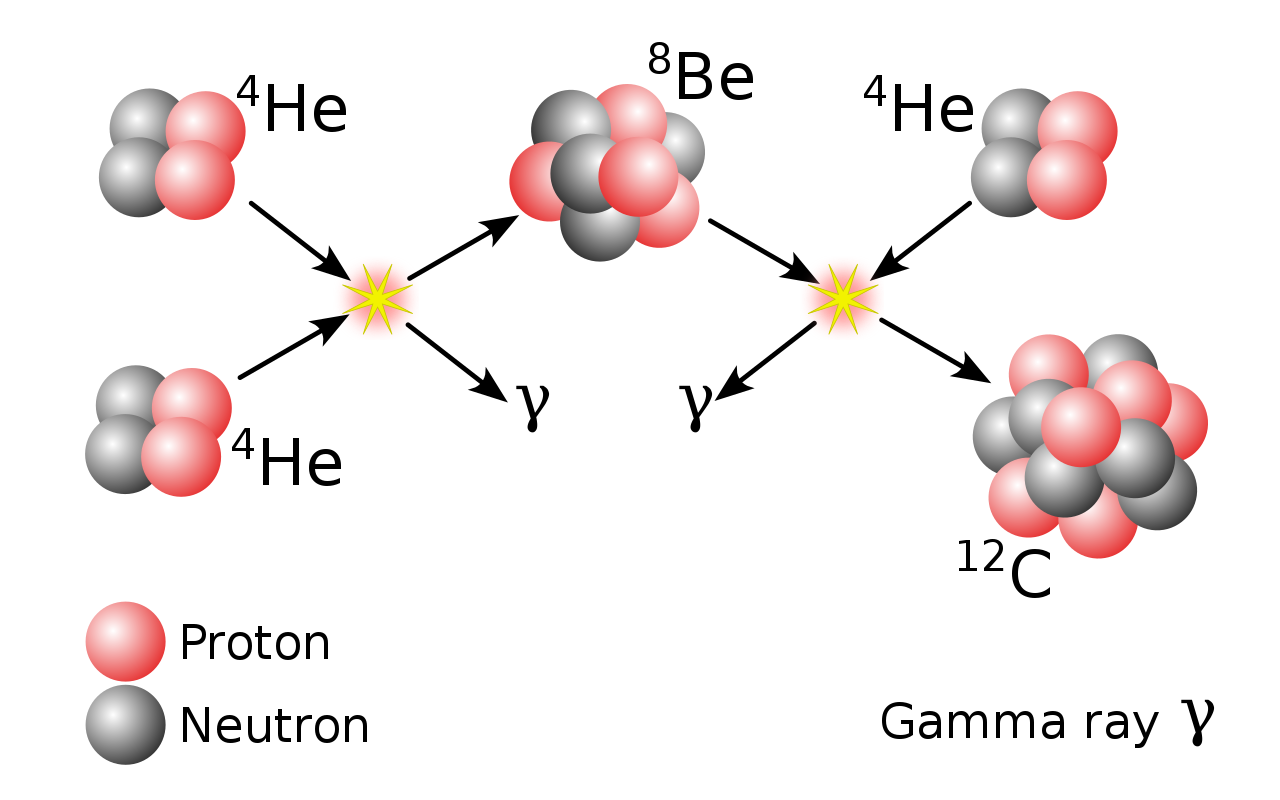
\includegraphics[width=0.5\textwidth]{graphics/sun/triple_alpha}
    \caption{Schematic of the triple-$\alpha$ process. Credit: \href{https://en.wikipedia.org/wiki/Triple-alpha_process}{Borb via English Wikipedia}.}
    \label{fig:sun:triple_alpha_process}
\end{figure}
The nuclear energy generation rate in W\,kg$^{-1}$ of the triple-$\alpha$ process, as described in \citet{carroll17} (equation (10.62) on page 312) is given as
\begin{equation}
    \epsilon_{3\alpha} = 50.9 \rho^{2} Y^{3} T_8^{-3} f_{3\alpha} \exp\left(-44.027 T_8^{-1}\right). \label{eqn:sun:triple_alpha_energy_generation}
\end{equation}
Here, $f_{3\alpha}$ is the screening factor for the triple-$\alpha$ process. Once enough carbon is produced, it becomes possible to capture another \ex{4}He on \ex{12}C, thus producing \ex{16}O in the reaction
\begin{equation}
    {^{12}}\mathrm{C} + {^4}\mathrm{He} \longrightarrow {^{16}}\mathrm{O} + \gamma.
\end{equation}

The energy release from fusing three \ex{4}He to \ex{12}C is 7.367\,MeV. While regularly, this additional energy would result in an expansion of the star, which would thus cool down and go into hydrostatic equilibrium again, the pressure does not rise in a degenerate gas. Thus, the temperature keeps rising, resulting in a vast acceleration of the triple-$\alpha$ process. This positive feedback loop results in a thermonuclear runaway, which ultimately ends in the so-called helium flash. The energy released during this helium flash does however not result in a stellar explosion but is rather used up in order to lift the degeneracy of the matter in the core, which subsequently yields a rapid expansion of the core. This expansion leads to a cooling in the hydrogen burning shell around the core, which has up to now been the sole supporter of the luminosity of the star. Thus, the Sun's luminosity drops significantly and it enters the horizontal branch on which it quietly burns helium in the core and hydrogen in a shell surrounding the core via the CNO cycle. This burning stage lasts for about 0.1\,Ga.

\paragraph{The \acl{agb}}
Once the helium in the core is exhausted, the Sun will have CO core in the center. The Sun will contract again until helium burning in a shell around the core starts. At the same time, hydrogen will be burning further out. The two areas are separated by an intershell region consisting mainly of helium. During this phase the Sun is on the \ac{eagb}. The \ac{agb} is named in this way since it asymptotically almost merges with the \ac{rgb}. The expanding and cooling star leads the convective envelope to again penetrate deeper, thus initiating the second dredge up. 

\paragraph{The \acl{tpagb}}
During the Sun's ascent of the \ac{agb}, helium burning becomes thermally unstable and the hydrogen and helium shells start burning alternatively. 
About 90\% of the time the hydrogen shell is burning, creating helium which subsequently increases the mass of helium and thus the temperature and pressure at the bottom of the intershell. At some point the temperature is high enough again to suddenly ignite helium burning at the bottom of the intershell, resulting in a thermal pulse. The Sun has now reached the \ac{tpagb} phase. 
The radius of the Sun varies by a factor of around four during this time and at its maximum radius can reach the Earth's orbit. Several of these thermal pulses will repeat at time intervals of around $10^5$\,a. Strong stellar winds during this period result in the Sun loosing a significant amount of mass. After about 20\,Ma in total, the Sun leaves the \ac{agb} branch.

\paragraph{Planetary nebula and white dwarf formation}
\begin{figure}[tb]
    \centering
    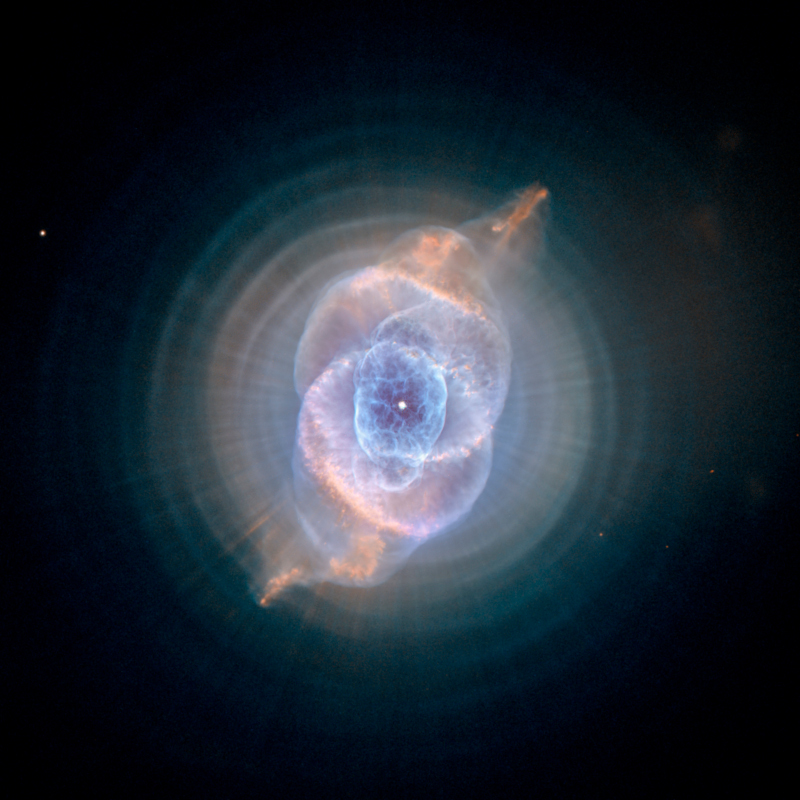
\includegraphics[width=0.6\textwidth]{graphics/sun/catseye_nebula}
    \caption{The Catseye Nebula -- a planetary nebula -- photographed with the Hubble space telescope. Credit: NASA, ESA, HEIC, and The Hubble Heritage Team (STScI / (AURA).}
    \label{fig:sun:catseye_nebula}
\end{figure}
As strong stellar winds continue, the Sun will lose enough mass to start loosing its hydrogen envelope. This exposes deeper and hotter layers, thus moving the star to the left in the \ac{hrd}. Once this surface temperature is high enough it will ionize the surrounding ejecta material via \ac{uv} radiation, making the material fluoresce brightly.
Figure~\ref{fig:sun:catseye_nebula} shows a Hubble image of the Catseye Nebula as an example of a \ac{pn}.

With ultimately all the hydrogen gone, the Sun itself will further contract until an electron degenerate CO \ac{wd} is left behind. At this point it weighs about half of its original mass. The gravitational force will be opposed by the degeneracy pressure. The \ac{wd} will continue to radiate heat away into space and thus slowly cool.


\section{The Death of More Massive Stars}

Intermediate mass stars ($2\,M_\odot < M < 11\,M_\odot$) will undergo a similar evolution to the one discussed for the Sun. During the \ac{tpagb} phase though, these stars will undergo multiple, so-called \ac{tdu} events. These events mix material from the intershell with the envelope. As we will see later, the \ac{sproc} takes place in the helium intershell. Thus, these \ac{tdu} events mix freshly nucleosynthesized material from the helium intershell into the convective envelope. Since the envelope gets ultimately ejected into space by stellar winds, \ac{sproc} material is effectively recycled into the Milky Way.

Stars more massive than $8\,M_\odot < M < 11\,M_\odot$ furthermore can successfully burn the carbon and oxygen further. The reactions that take place for carbon burning are the following:
\begin{equation}
    {^{12}}\mathrm{C} + {^{12}}\mathrm{C} \longrightarrow 
    \begin{cases}
        {^{16}}\mathrm{O} + 2\,{^4}\mathrm{He} \quad &(*)\\
        {^{20}}\mathrm{Ne} + {^4}\mathrm{He}\\
        {^{23}}\mathrm{Na} + p^+\\
        {^{23}}\mathrm{Mg} + n \quad &(*)\\
        {^{24}}\mathrm{Mg} + \gamma
    \end{cases}
\end{equation}
For oxygen burning, the reactions are:
\begin{equation}
{^{16}}\mathrm{O} + {^{16}}\mathrm{O} \longrightarrow 
    \begin{cases}
        {^{24}}\mathrm{Mg} + 2\,{^4}\mathrm{He} \quad & (*)\\
        {^{28}}\mathrm{Si} + {^4}\mathrm{He}\\
        {^{31}}\mathrm{P} + p^+\\
        {^{31}}\mathrm{S} + n\\
        {^{32}}\mathrm{S} + \gamma
    \end{cases}
\end{equation}
Note that reactions labeled with (*) in fact consume energy and do not produce any. This behavior is however enabled by the high temperatures present during CO burning. Instead of a CO \ac{wd}, stars in this mass range leave behind a ONe \ac{wd}

Stars more massive than $11\,M_\odot$ undergo further burning reactions and end up in their final state as either neutron stars or black holes. These massive stars -- at least some -- are also expected to explode as \acp{sn}. We will discuss their fate further in the next chapter.


\section{Stellar Lifetimes}

While the quiescent burning of the Sun takes place over around 10\,Ga, subsequent burning phases are exponentially faster. The total life of the Sun is thus defined by the quiescent burning phase. This can be generalized to other stars. If the mass of a star increases, the central pressure and temperature will necessarily go up as can be seen in equations~\eqref{eqn:star_formation:central_pressure} and~\eqref{eqn:star_formation:central_temperature}, respectively. Thus, the nuclear fuel will burn faster resulting in a higher luminosity of the star. From observations of main sequence stars, an empirical mass-luminosity relation can be determined approximately as
\begin{equation}
    L = L_\odot \left(\frac{M}{M_\odot}\right)^{3.5}. \label{eqn:sun:mass_luminosity_relation}
\end{equation}

The lifetime of a star is proportional to its luminosity divided by its mass since the mass is proportional to the amount of fuel. We can therefore roughly estimate the lifetime dependency in comparison to the solar lifetime with respect to a star's mass. The dependency yields
\begin{equation}
    t_\mathrm{nuc}(M) \approx t_{\odot\mathrm{,total}} \left(\frac{M_\odot}{M}\right)^{2.5}. \label{eqn:sun:stellar_lifetime_estimate}
\end{equation}
This equation should solely be used for back-of-the-envelope-type calculations, however, it helps to understand the fact that more massive stars die faster. Detailed determinations of the stellar lifetimes require adequate models that include the energy generation equations, e.g., equations~\eqref{eqn:sun:energy_generation_pp-chain} and~\eqref{eqn:sun:energy_generation_cno_cycle}, as well as an accurate thermodynamic model of the inside of a star.

\section{Reading}

In this chapter we have in detail discussed the inner workings of the Sun. The reading chosen to supplement our theoretical understanding of the Sun discusses the experimental work that went into actually observing the quiescent burning using neutrino detectors.

Please read \citet{davis55} and \citet{bahcall76}. We will briefly discuss \citet{davis55} and these pioneering measurements and then focus on \citet{bahcall76}. The following points might help to guide the reading:
\begin{itemize}
    \item What is the general understanding of neutino research in 1955? How does this influence the hypothesis of \citet{davis55}?
    \item Discuss the experimental setup of \citet{davis55}. It might help to make a drawing of the setup to the best of your understanding. Split the setup up into two parts, (1) how to get \ex{37}Ar out of the tank and (2) how it is subsequently detected.
    \item What are the (stunning) conclusions of \citet{davis55}?
    \item How has the knowledge of neutrinos changed in between \citet{davis55} and \citet{bahcall76}?
    \item What neutrinos can be detected with the experiment of \citet{bahcall76}? Which reactions do these neutrinos originate from? Put your findings into context of Figure~\ref{fig:sun:pp-chain}.
    \item What is different in the experimental setup disucssed in \citet{bahcall76} compared to \citet{davis55}?
    \item Discuss why the experiment described in \citet{bahcall76} was performed underground? Compare the Homestake mine to other underground laboratories. Was the shielding of the mountain enough to achieve the required sensitivity?
    \item How did the experimentalists ensure that their result is correct?
    \item What solar processes can be excluded from these measurements? Where lies the solar neutrino problem?
    \item What alternative explanations are given by \citet{bahcall76} that might solve the solar neutrino problem?
    \item Who won in the end, the astronomers or the physicists? What implication did this finding have -- for the world and for Ray Davis?
\end{itemize}